%% $RCSfile: proj_report_outline.tex,v $
%% $Revision: 1.3 $
%% $Date: 2016/06/10 03:41:54 $
%% $Author: kevin $

\documentclass[11pt
              , a4paper
              , twoside
              , openright
              ]{report}


\usepackage{float} % lets you have non-floating floats

\usepackage{url} % for typesetting urls

\usepackage{soul}
\usepackage{color}

%
%  We don't want figures to float so we define
%
\newfloat{fig}{thp}{lof}[chapter]
\floatname{fig}{Figure}

%% These are standard LaTeX definitions for the document
%%                            
\title{aWall: Adding Collaboration Support for Agile Retrospectives}
\author{Simon Glew}

%% This file can be used for creating a wide range of reports
%%  across various Schools
%%
%% Set up some things, mostly for the front page, for your specific document
%
% Current options are:
% [ecs|msor|sms]          Which school you are in.
%                         (msor option retained for reproducing old data)
% [bschonscomp|mcompsci]  Which degree you are doing
%                          You can also specify any other degree by name
%                          (see below)
% [font|image]            Use a font or an image for the VUW logo
%                          The font option will only work on ECS systems
%
\usepackage[image,ecs,behons]{vuwproject} 

% You should specifiy your supervisor here with
%     \supervisor{Firstname Lastname}
% use \supervisors if there is more than one supervisor
\supervisor{Dr. Craig Anslow}

% Unless you've used the bschonscomp or mcompsci
%  options above use
%   \otherdegree{OTHER DEGREE OR DIPLOMA NAME}
% here to specify degree

% Comment this out if you want the date printed.
\date{}

\begin{document}

% Make the page numbering roman, until after the contents, etc.
\frontmatter

%%%%%%%%%%%%%%%%%%%%%%%%%%%%%%%%%%%%%%%%%%%%%%%%%%%%%%%

%%%%%%%%%%%%%%%%%%%%%%%%%%%%%%%%%%%%%%%%%%%%%%%%%%%%%%%

\begin{abstract}

Agile does not have an online tool that allows integration to different online tools and allowing users to use this integration when participating in agile retrospectives. It is a problem as it means either the team has to be co-located or use the addition of different third-party applications such as Skype. By creating and integrating online retrospective tools within aWall will allow users to participate in agile retrospectives online within the tool. This report outlines the overall project that was carried out including the planning, implementation and evaluation of the tool.

\end{abstract}

%%%%%%%%%%%%%%%%%%%%%%%%%%%%%%%%%%%%%%%%%%%%%%%%%%%%%%%

\maketitle

\chapter*{Acknowledgments}\label{C:ack} 
Any acknowledgments should go 
in here, between the title page and the table of contents.  The 
acknowledgments do not form a proper chapter, and so don't get a 
number or appear in the table of contents.

\tableofcontents

% we want a list of the figures we defined
\listof{fig}{Figures}

%%%%%%%%%%%%%%%%%%%%%%%%%%%%%%%%%%%%%%%%%%%%%%%%%%%%%%%

\mainmatter

%%%%%%%%%%%%%%%%%%%%%%%%%%%%%%%%%%%%%%%%%%%%%%%%%%%%%%%

% individual chapters included here
\chapter{Introduction}\label{C:intro}
\section{The Problem} 
The problem that this project is to solve is attempting to support agile retrospectives meetings through touch walls and screens, this is going to be done by creating a prototype application that will be used to support them. This project is part of the aWall software project run by Dr. Craig Anslow and Professor Martin Kropp of FHNW in Switzerland. Agile Retrospectives are meetings held within teams once complementing an increment of work. They allow teams to inspect and adapt the different areas that are required within themselves and allow for change and learning within the entire team\cite{AgileRetrospectivesEstherDerby}.

The outcome of this project, is to build a software web system to help facilitate agile retrospective meetings using a large touch screen as an output for the software. Once this software has been built, an evaluation with users will occur to evaluate and improve on the software project. The current aWall project can be found here: \url{https://www.youtube.com/watch?v=fzCnjnpRiTI}

\begin{figure}[ht]
\centering
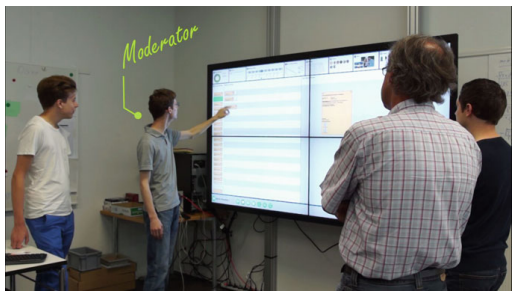
\includegraphics{aWall_introduction}
\caption{Project aWall - digital agile cardwall being used \cite{xp2017_aWall}}
\end{figure}

\section{Overview of Research Project}
This project will be building off this current prototype but within its own project scope and no integration between the two codebases.

This software prototype is split into three different components:
\begin{itemize}
\item \textbf{Participant System:} The participant system is used for the participants to interact within the system, it is an application that will allow the participant to vote and make notes about the retrospective and directly interact with what is happening on the screen and within the retrospective. All the interactions from this system get seny and stored within the database housed within the server. This system will be accessed from a secondary device by the user e.g their phone. This system sets up a connection to the server through a socket, allowing for the required transfer of data.
\item \textbf{Screen System:} The screen system is an application that the moderator of the retrospective interacts with, it allows the moderator to display and manipulate the data passed from the server that the participants have given. This system will be used on the touch screen with a connection to the server through a socket.  
\item \textbf{Server:} The server houses all the data storage and manipulation for the overall software system. The server also houses the socket system allowing for real-time updates between the participant and screen systems. The server allows the storage of data for futher use in later iterations of the projects lifecycle, e.g. a later agile retrospective. 
\end{itemize}

Within this prototype there will be different versions of agile retrospectives that the different members of the agile team can choose. The different retrospectives that were chosen through doing a background review on the different retrospectives methods that where found. The ones that were chosen either linked up with the other two sections of a retrospective nicely or were found within multiple different sources \cite{AgileRetrospectivesEstherDerby, normanKeith}. The retrospective methods that were chosen are:
\begin{itemize}
\item The 3W's/Mad, Sad and Glad
\item Timeline
\item Brainstorm/Filtering
\item Short Subjects
\end{itemize}

Each of these retrospective methods will be able to be selected from the screen system within the software application when creating a retrospective session. To accompany each of these retrospective methods, there will also be short sections before and after the main method, it allows for the setting of the scene within the retrospective and to wrap up the retrospective also.

The methods that I have chosen for this are:  \cite{AgileRetrospectivesEstherDerby}
\begin{itemize}
\item \textbf{Setting the scene:} Check-in
\item \textbf{Wrapping-up:} +/- or Delta
\end{itemize}

Using each of these methods, I will be able to evaluate the best retrospective method through conducting user testing using all of the methods above.

\chapter{Background Review and Related Work}\label{C:background}
Retrospectives are meetings held within agile teams, involving all members of the team and is held at the end and just after an iteration of work \cite{AgileRetrospectivesEstherDerby,GettingValueFromRetrospectives}. The retrospective is used for not only celebrating the success of work from the last retrospective, but also the failures and lessons that can be learnt from them \cite {normanKeith}. The retrospective is normally facilitated by a third party member who does not have a personal stake in the in the content or outcome of the meeting, therefore being able to remain neutral during the meeting \cite{normanKeith,retrospectiveFacilator}. Retrospectives are used to reflect on the work done since the last retrospective and the problems that the team faced within this work. \cite{AgileRetrospectivesEstherDerby}. aWall is a online tool that allows for collaboration within a team when it comes to agile practices \cite{xp2017_aWall}, including the aqile practice of retrospectives. With the tool being online, it allows teams to seperate members while still all members can include thoughts and feelings to the agile practices within the team.  

\textbf{NEEDS MORE WORK - WILL DO LATER THIS WEEK, WITH SPLIT INTO SECTIONS}
\section{Agile and Agile Retrospectives}
\section{aWall}
\chapter{Design}\label{C:design}

\chapter{Implementation}\label{C:implementation}

\chapter{Evaluation of Solution}\label{C:evalution}
The solution is going to be evaluated through User Studies. A ethics proposal has been submitted to the Human Ethics Committee within Victoria and is currently going through the process of being evaluated and approved, the ethics application number is \textit{\#0000026187}. 
\section{Process}
The process for the user study will consist of the following steps:
\begin{itemize}
\item Users will volunteer and be placed into groups or 'teams' to do the retrospectives in.
\item The teams will firstly participate within a 'control' retrospective, where they will do part of a retrospective the old way, using a cardwall.
\item The teams will then participate in a retrospective using the aWall tool using one of the 4 main retrospective methods
\item Finally the members within each of the teams will fill out a questionnaire about the experience, the questionnaire can been seen in the Appendices as Appendix One. 
\end{itemize}

Using the data gathered from the questionnaires and from the observations within the user study, I will be able to not only evaluate the success of using a touch wall over a card wall, but also what retrospective method has the greatest engagement within different software teams. 

\chapter{Conclusions and Future Work}\label{C:con}
The conclusions are presented in this Chapter.



%%%%%%%%%%%%%%%%%%%%%%%%%%%%%%%%%%%%%%%%%%%%%%%%%%%%%%%

\backmatter

%%%%%%%%%%%%%%%%%%%%%%%%%%%%%%%%%%%%%%%%%%%%%%%%%%%%%%%


%\bibliographystyle{ieeetr}
\bibliographystyle{acm}
\bibliography{sample}


\end{document}
